% !TEX root=main.tex

We are now in a position to empirically compare the methods discussed above,
to get a firmer sense of their tradeoffs.

%
\subsection{Description of datasets}

We used the trajectory data\footnote{\url{https://bitbucket.org/d-chen/tour-cikm16}}
extracted from Flickr photos for the cities of Glasgow, Osaka and
Toronto~\cite{ijcai15,cikm16paper}.
Each dataset comprises of a
list of trajectories, being a sequence of points of interest (POI),
as visited by various Flickr users and recorded by the geotags in photos.
Table~\ref{tab:data} summarises the profile of each dataset.
We see that most queries have more than one ground truth, making the sequence recommendation setting relevant. Further, each query has an average of 4-9, and a maximum of 30-60 trajectories (details in supplement).

% In all datasets,
% each user has on average less than two trajectories.
% This makes user-specific recommendation impractical, and also undesirable because
% a user would want different recommendations given different starting locations, and not a static recommendation no matter where she is.

% dataset stats
% \begin{table}[t]
% 	\begin{minipage}[t]{\linewidth}
% 		\resizebox{\linewidth}{!}{
% 		\setlength{\tabcolsep}{4pt} % tweak the space between columns
% 		\small
% 		\begin{tabular}{lllll|ccc|cc} \hline %{l*{9}{c}} \hline
% 		\textbf{Dataset} & \textbf{\#Traj} & \textbf{\#POIs} & \textbf{\#Users} & \textbf{\#Queries} & \textbf{\#GT=1} & \textbf{\#GT$\in [2,5]$} & \textbf{\#GT$>$5} & \textbf{\#shortTraj} & \textbf{\#longTraj} \\ \hline
% 		Glasgow          & 351              & 25              & 219              & 64                 & 23              & 22                      & 19                & 336                     & 15 \\
% 		Osaka            & 186              & 26              & 130              & 47                 & 17              & 22                      & 8                 & 178                     & 8  \\
%         Toronto          & 977              & 27              & 454              & 99                 & 30              & 33                      & 36                & 918                     & 59 \\
% 		\hline
% 		\end{tabular}%
% 		}
% 		\captionof{table}{Statistics of trajectory datasets.
%         Including the number of trajectories (\#Traj), POIs (\#POIs), users (\#Users), queries (\#Queries);
%         the number of queries with a single (\#GT=1), 2-5 (\#GT$\in$[2,5]), or more than 5 (\#GT$>$5) ground truths;
%         and profile of trajectory length, \ie less than 5 (\#shortTraj) and more than 5 POIs (\#longTraj).
%         }
% 		\label{tab:data}
% 	\end{minipage}
% \end{table}

\begin{table}[t]
	\begin{minipage}[t]{\linewidth}
		\resizebox{\linewidth}{!}{
		\setlength{\tabcolsep}{4pt} % tweak the space between columns
		\small
		\begin{tabular}{llll|cc} \hline %{l*{9}{c}} \hline
		\textbf{Dataset} & \textbf{\#Traj} & \textbf{\#POIs}  & \textbf{\#Queries}  & \textbf{\#ShortTraj} & \textbf{\#LongTraj} \\ \hline
		Glasgow          & 351              & 25              & 64                 & 336                     & 15 \\
		Osaka            & 186              & 26              & 47                 & 178                     & 8  \\
        Toronto          & 977              & 27              & 99                 & 918                     & 59 \\
		\hline
		\end{tabular}%
		}
		\captionof{table}{Statistics of trajectory datasets.
        Including the number of trajectories (\#Traj), POIs (\#POIs), queries (\#Queries);
        and the number of trajectories with length less than 5 (\#ShortTraj) and more than 5 POIs (\#LongTraj).
        }
		\label{tab:data}
	\end{minipage}
\end{table}

%
\subsection{Experimental protocol}

We compare the three methods described previously ({\sc List Viterbi}, {\sc ILP}, {\sc LoopElim}),
as well as the standard inference ({\sc Viterbi}).

We evaluate each algorithm using leave-one-query-out cross validation (LOOCV).
That is, holding out all the relevant trajectories for each query $\x^{(i)}$ (\ie $\{\y^{(i,j)}\}_{j=1}^{n_i}$) in each round.
The regularisation constant $C$ is tuned using Monte Carlo cross validation~\cite{burman1989comparative} on the training set.
We use three performance measures for POIs, sequences and ordered lists.
The {\bf F$_1$ score on points}~\cite{ijcai15} computes F$_1$ on the predicted versus seen points
without considering their relative order.
The {\bf F$_1$ score on pairs}~\cite{cikm16paper} is proposed to mitigate this by computing F$_1$ on all ordered pairs in the predicted versus ground truth sequence. %%It is 1 iff both sequences agree completely.
%The well-known rank correlation {\bf Kendall's $\tau$}~\cite{agresti2010analysis}
%computes the ratio of concordant (correctly ranked) pairs minus discordant pairs, over all possible pairs after accounting for ties.%taking care of ties.


%
\subsection{Results and discussion}

We now address the motivating questions of this work.

\textbf{How often does the top-scoring sequence have loops?}
It is first of interest to determine that the top-scoring sequence for the underlying SSVM model does in fact often contain loops.
We find that on the (Osaka, Glasgow, Toronto) datasets, the top-scoring sequence for (23.9\%, 31.2\%, 48.5\%) respectively of all queries have loops.
This confirms that with longer trajectories, even a powerful structured model cannot escape the problem of predicting sequences with loops.

% Osaka percentage of predictions with loops:
% 11 / 46 = 23.9\% \\
% Glasgow percentage of predictions with loops:
% 20 / 64 = 31.2\% \\
% Toronto percentage of predictions with loops:
% 48 / 99 = 48.5\% 

\textbf{How important is it to remove loops?}
Having confirmed that loops in the top-scoring sequence are an issue,
it is now of interest to establish that removing such loops during prediction is in fact important.
This is confirmed in Tables \ref{tab:f1-master} -- \ref{tab:pf1-master},
where we see that there can be as much as a 50\% improvement in performance over the {\sc Viterbi} baseline.

\textbf{How reliably can {\sc LoopElim} get the desired length?}
A challenge in applying {\sc LoopElim} to the trajectory recommendation problem as we have defined it
is that it may result in a trajectory of the wrong length.
Figure \ref{fig:length-christo} shows that a significant fraction of queries will have a different length to the target.

\textbf{How reliably can {\sc LoopElim} predict a good trajectory?}
Assuming one can overlook the {\sc LoopElim} producing a trajectory of possibly incorrect length,
it is then of interest as to how well it performs compared to the list Viterbi and ILP methods.
Tables \ref{tab:f1-master} -- \ref{tab:pf1-master} show that the heuristic, while sometimes competitive on the F1 measures, often
grossly underperforms compared to the more principled approaches.

%Interestingly, if Kendall's $\tau$ is the measure of interest, then the heuristic may actually be preferable to these methods.

\textbf{Which of ILP or list Viterbi is faster, and when?}
The list Viterbi and ILP methods have highly similar accuracy, with the differences owing to ties.
What about their relative runtimes?
Figure \ref{fig:inftime} shows that for shorter trajectories, the list Viterbi approach is to be preferred;
however, for longer trajectories, the ILP approach is faster.

The reason for the list Viterbi to suffer at longer trajectories is simply because this creates an exponential increase in the number of available choices, which must be searched through serially.
Of interest is that ILP approach has runtime largely independent of the trajectory length.
This indicates the branch-and-bound as well as cutting plane underpinnings of these solvers are highly scalable.

As a final note, we see that the complexity of the LoopElim is several order of magnitudes less than either of the two more advanced methods at longer trajectories.
There is thus a familiar tradeoff between time and accuracy.

% !TEX root = ./main.tex

\begin{table*}[t]\captionmoveup
     \caption{Results on trajectory recommendation datasets on best of top-10.
     %The top three rows are baselines, and the bottom four are the methods proposed in this paper.
     Higher scores are better for all metrics. Bold entries: \textbf{best} performing method for each metric; italicised entries: the \textit{second best}.
     }
     \label{tab:result}
     \centering
%%     \setlength{\tabcolsep}{3pt} % tweak the space between columns
%%     \small
     \resizebox{\linewidth}{!}{
%%     \begin{tabular}{l|cc|cc|cc} \hline
%%                         & \multicolumn{2}{|c}{\textbf{Kendall's $\tau$}}
%%                         & \multicolumn{2}{|c}{\textbf{F$_1$ score on points}}
%%                         & \multicolumn{2}{|c}{\textbf{F$_1$ score on pairs}} \\ \cline{2-7}
%%                         & Osaka & Glasgow
%%                         & Osaka & Glasgow
%%                         & Osaka & Glasgow \\ \hline
%%     \textsc{Random}     & $0.685\pm0.035$ & $0.703\pm0.029$
%%                         & $0.703\pm0.032$ & $0.731\pm0.026$
%%                         & $0.451\pm0.057$ & $0.495\pm0.046$ \\
%%     \textsc{Popularity} & $0.768\pm0.038$ & $0.748\pm0.036$
%%                         & $0.786\pm0.034$ & $0.771\pm0.033$
%%                         & $0.626\pm0.055$ & $0.623\pm0.051$ \\
%%     \textsc{PoiRank}    & $0.787\pm0.037$ & $0.830\pm0.029$
%%                         & $0.804\pm0.034$ & $0.847\pm0.025$
%%                         & $0.661\pm0.056$ & $0.726\pm0.043$ \\
%%     \midrule
%%     \textsc{SP}         & $0.749\pm0.043$ & $0.790\pm0.030$
%%                         & $0.770\pm0.039$ & $0.810\pm0.027$
%%                         & $0.620\pm0.061$ & $0.658\pm0.046$ \\
%%     \textsc{SPpath}     & $\mathit{0.791\pm0.036}$ & $0.787\pm0.029$
%%                         & $\mathit{0.809\pm0.033}$ & $0.807\pm0.026$
%%                         & $\mathit{0.664\pm0.055}$ & $0.648\pm0.045$ \\
%%     \textsc{SR}         & $0.777\pm0.036$ & $\mathbf{0.868\pm0.026}$
%%                         & $0.793\pm0.033$ & $\mathbf{0.883\pm0.023}$
%%                         & $0.637\pm0.055$ & $\mathbf{0.770\pm0.039}$ \\
%%     \textsc{SRpath}     & $\mathbf{0.803\pm0.034}$ & $\mathit{0.853\pm0.026}$
%%                         & $\mathbf{0.820\pm0.031}$ & $\mathit{0.868\pm0.023}$
%%                         & $\mathbf{0.671\pm0.053}$ & $\mathit{0.746\pm0.041}$ \\ \hline
%%     \end{tabular}
\begin{tabular}{l|cc|cc|ccc} \hline
& \multicolumn{7}{c}{\bf Kendall's $\tau$} \\ \hline
 & \textsc{Random} & \textsc{Popularity} & \textsc{PoiRank} & \textsc{SP} & \textsc{SPpath} & \textsc{SR} & \textsc{SRpath} \\ \hline
Glasgow & $0.703\pm0.029$ & $0.748\pm0.036$ & $0.830\pm0.029$ & $0.790\pm0.030$ & $0.787\pm0.029$ & $\mathbf{0.868\pm0.026}$ & $\mathit{0.853\pm0.026}$ \\
Osaka & $0.685\pm0.035$ & $0.768\pm0.038$ & $0.787\pm0.037$ & $0.749\pm0.043$ & $\mathit{0.791\pm0.036}$ & $0.777\pm0.036$ & $\mathbf{0.803\pm0.034}$ \\
Toronto & $0.652\pm0.024$ & $0.719\pm0.024$ & $0.784\pm0.023$ & $0.697\pm0.027$ & $0.719\pm0.026$ & $\mathbf{0.802\pm0.022}$ & $\mathit{0.797\pm0.022}$ \\
\hline
& \multicolumn{7}{c}{\bf F$_1$ score on points} \\ \hline
Glasgow & $0.731\pm0.026$ & $0.771\pm0.033$ & $0.847\pm0.025$ & $0.810\pm0.027$ & $0.807\pm0.026$ & $\mathbf{0.883\pm0.023}$ & $\mathit{0.868\pm0.023}$ \\
Osaka & $0.703\pm0.032$ & $0.786\pm0.034$ & $0.804\pm0.034$ & $0.770\pm0.039$ & $\mathit{0.809\pm0.033}$ & $0.793\pm0.033$ & $\mathbf{0.820\pm0.031}$ \\
Toronto & $0.696\pm0.021$ & $0.746\pm0.022$ & $0.807\pm0.020$ & $0.733\pm0.023$ & $0.755\pm0.022$ & $\mathbf{0.828\pm0.019}$ & $\mathit{0.823\pm0.020}$ \\
\hline
& \multicolumn{7}{c}{\bf F$_1$ score on pairs} \\ \hline
Glasgow & $0.495\pm0.046$ & $0.623\pm0.051$ & $0.726\pm0.043$ & $0.658\pm0.046$ & $0.648\pm0.045$ & $\mathbf{0.770\pm0.039}$ & $\mathit{0.746\pm0.041}$ \\
Osaka & $0.451\pm0.057$ & $0.626\pm0.055$ & $0.661\pm0.056$ & $0.620\pm0.061$ & $\mathit{0.664\pm0.055}$ & $0.637\pm0.055$ & $\mathbf{0.671\pm0.053}$ \\
Toronto & $0.438\pm0.034$ & $0.550\pm0.035$ & $0.649\pm0.033$ & $0.530\pm0.037$ & $0.552\pm0.036$ & $\mathbf{0.660\pm0.033}$ & $\mathit{0.657\pm0.034}$ \\
\hline
\end{tabular}
     }\eqmoveup
\end{table*}


\begin{figure*}[!t]
\begin{minipage}[c]{0.8\textwidth}
%\begin{figure*}[!t]
		\centering
		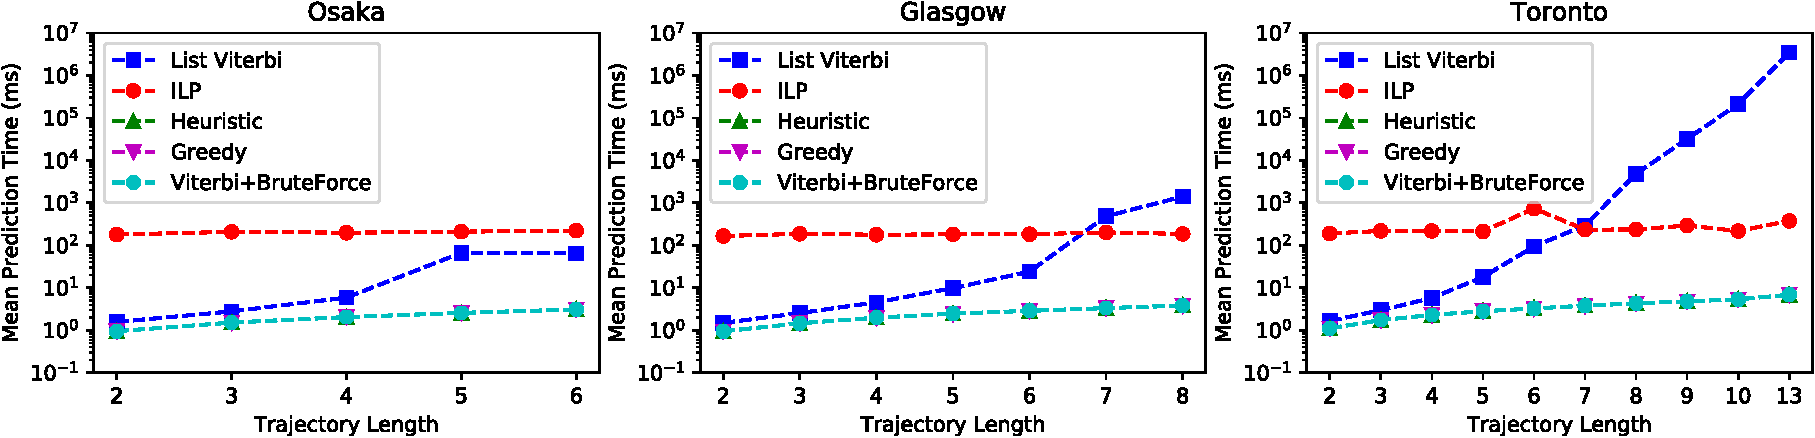
\includegraphics[width=\textwidth]{top1_inftime.pdf}
	    \captionof{figure}{Prediction time for three inference algorithms (in milliseconds)}
	    \label{fig:inftime}
	    %\captionmoveup\eqmoveup
%\end{figure*}%
%\begin{figure*}[!t]
		\quad
		\centering
		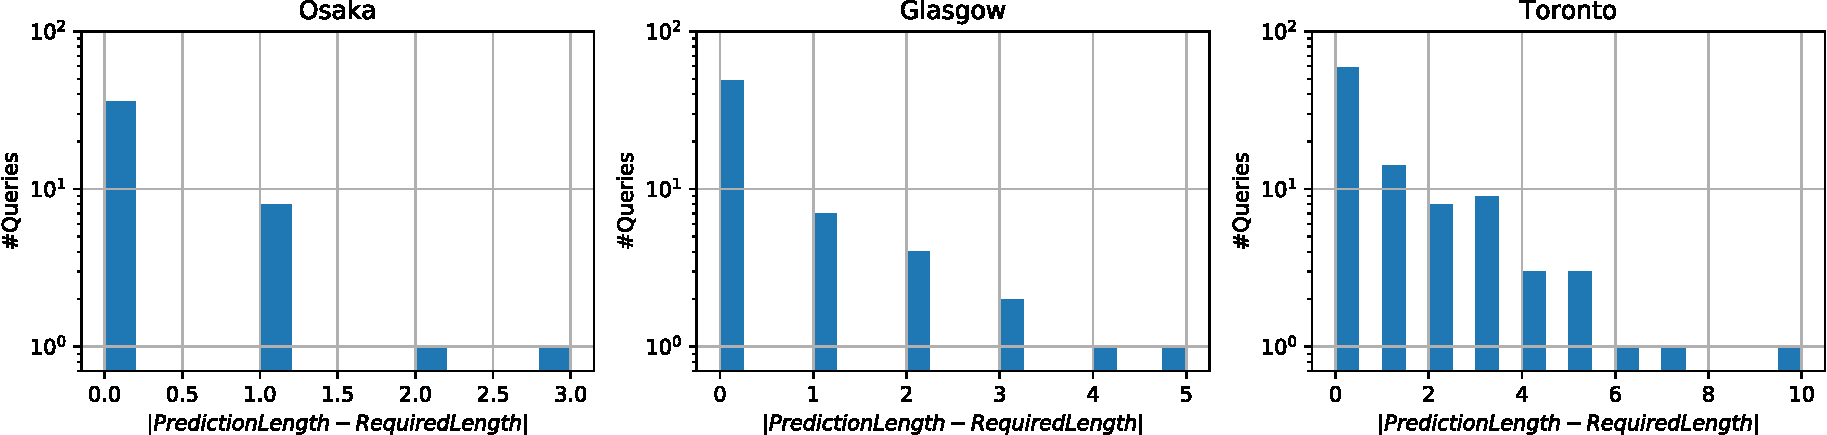
\includegraphics[width=\textwidth]{heu_lengthdiff.pdf}
	    \captionof{figure}{The difference between recommendation and required sequence length.}
	    \label{fig:length-christo}
	    %\captionmoveup\eqmoveup
%\end{figure*}%
%\begin{figure*}[!t]
		\quad
		\centering
		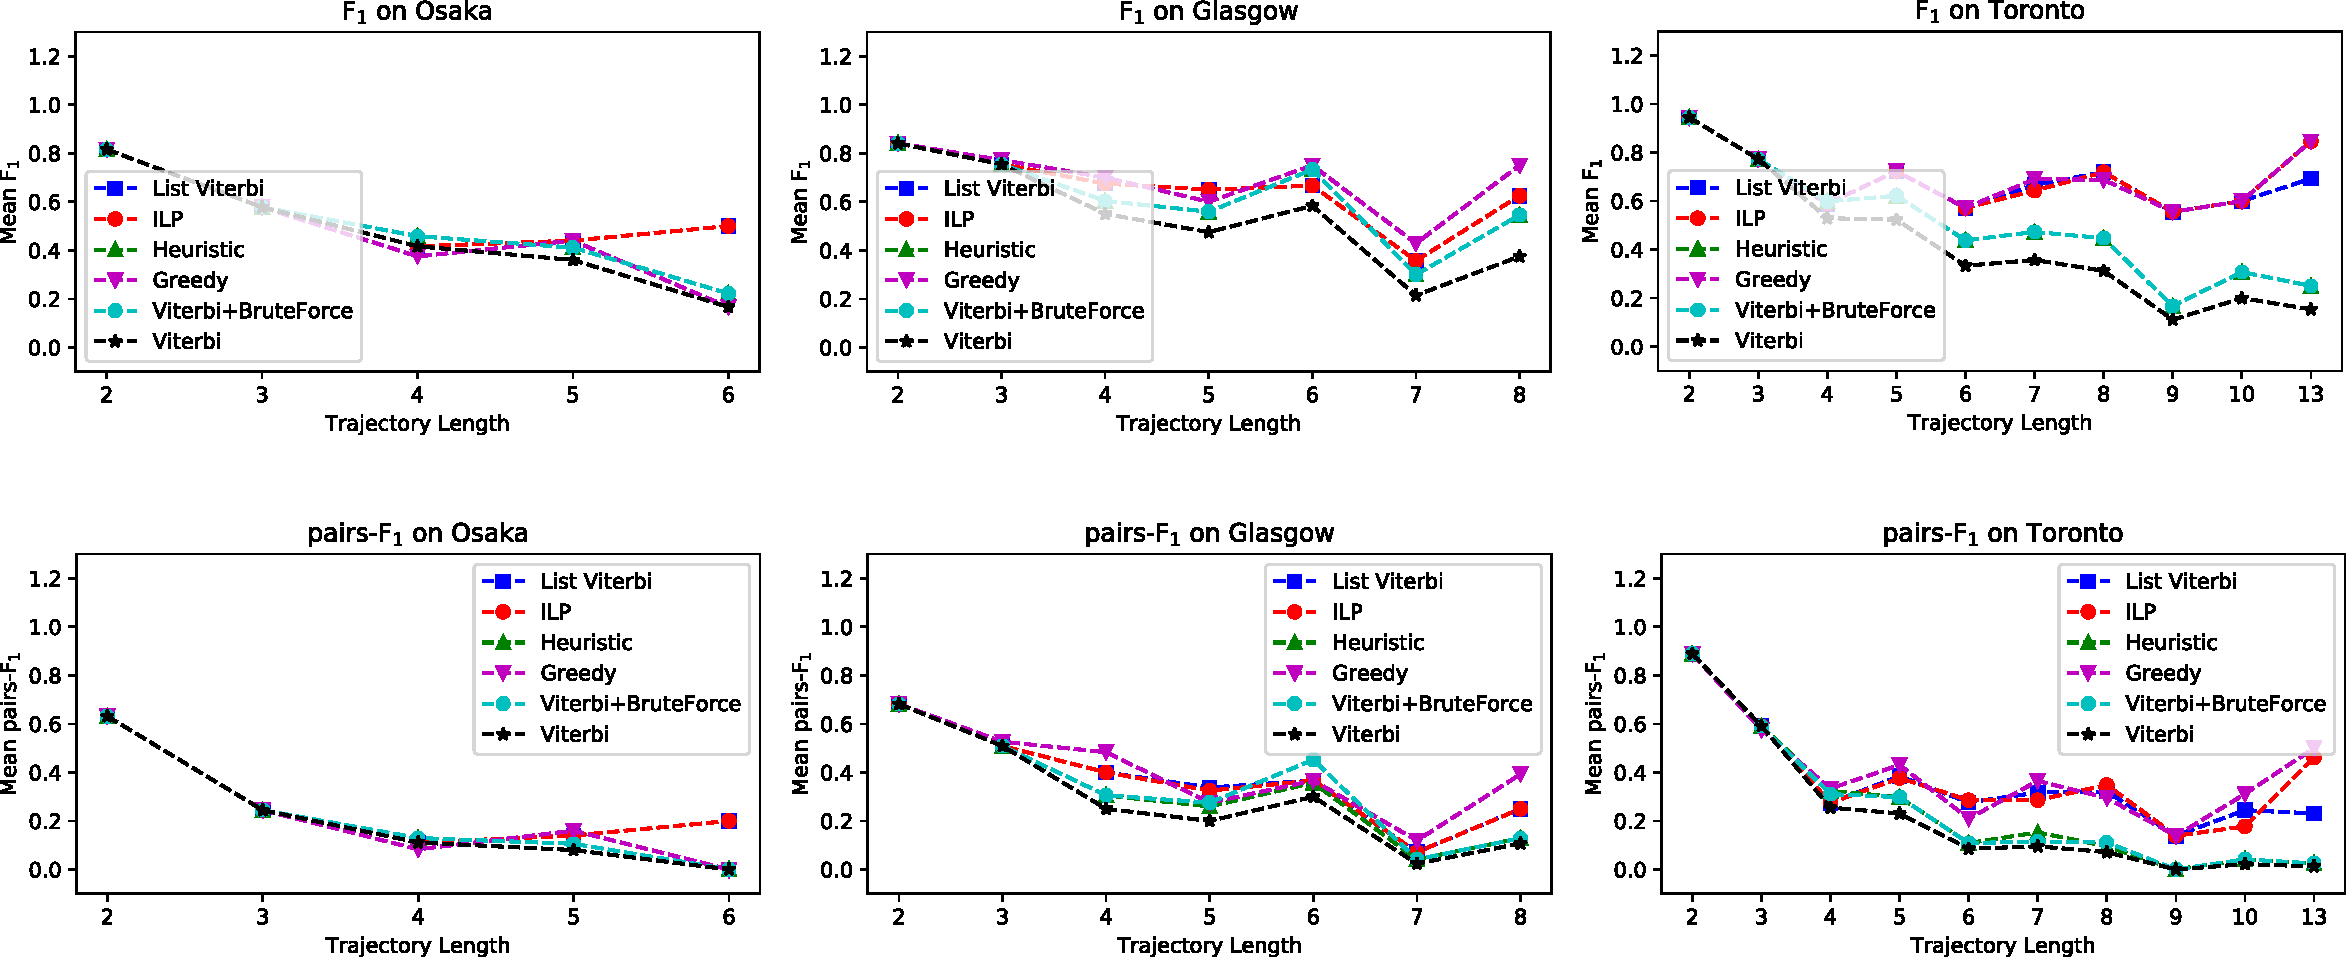
\includegraphics[width=\textwidth]{metrics.pdf}
		% 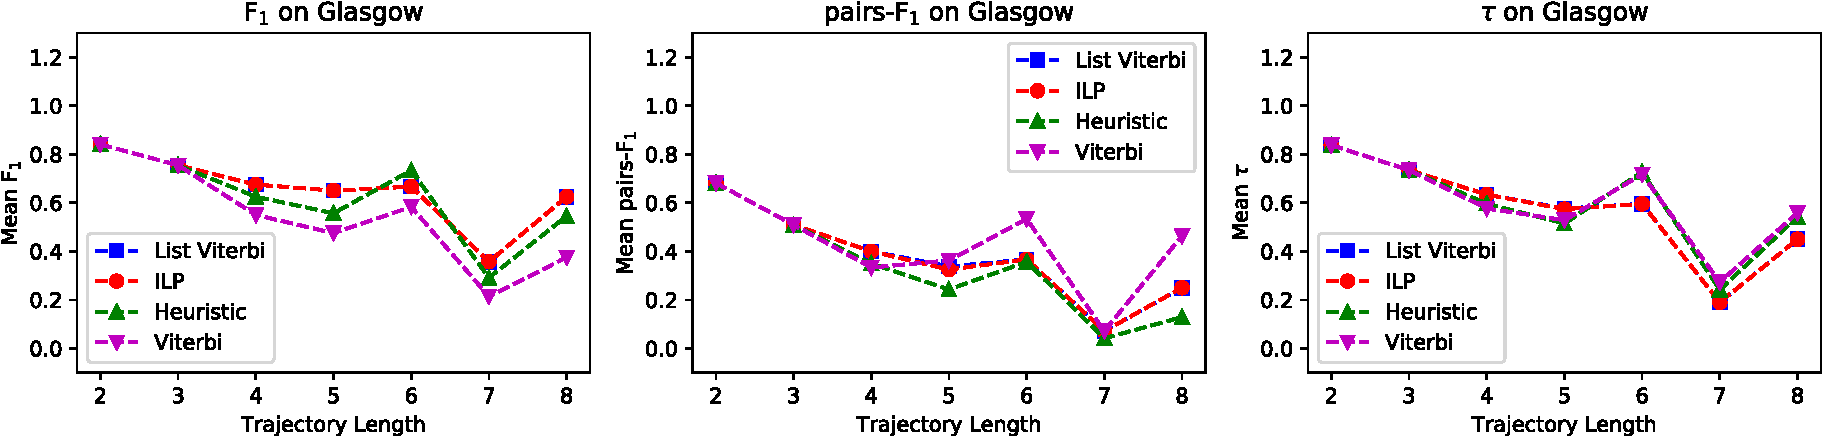
\includegraphics[width=\textwidth]{metric_d2.pdf}
		% 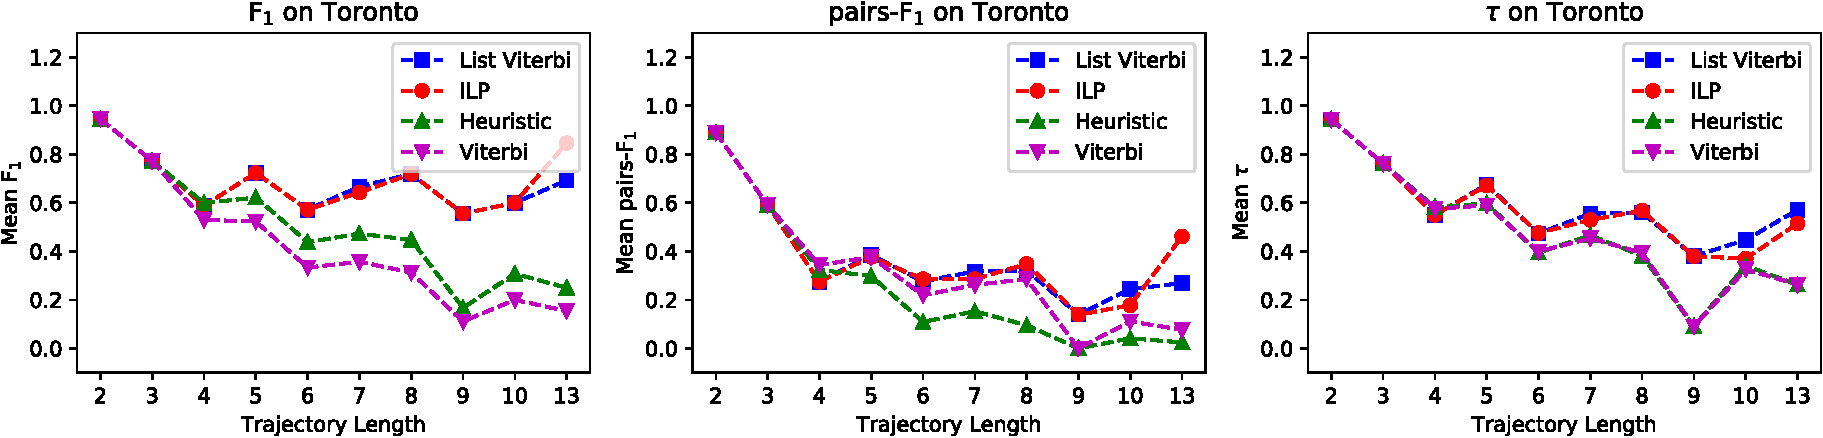
\includegraphics[width=\textwidth]{metric_d3.pdf}
	    \captionof{figure}{Accuracy versus trajectory length.}
	    \label{fig:acc-vs-length}
	    %\captionmoveup\eqmoveup
%\end{figure*}
\end{minipage}
\end{figure*}
